\documentclass[12pt,twoside]{article}
\usepackage[dvipsnames]{xcolor}
\usepackage{amsmath}
\usepackage{tikz,graphicx,amsmath,amsfonts,amscd,amssymb,bm,cite,epsfig,epsf,url}
\usepackage[hang,flushmargin]{footmisc}
\usepackage[colorlinks=true,urlcolor=blue,citecolor=blue]{hyperref}
\usepackage{amsthm,multirow,wasysym,appendix}
\usepackage{array,subcaption} 
% \usepackage[small,bf]{caption}
\usepackage{bbm}
\usepackage{pgfplots}
\usetikzlibrary{spy}
\usepgfplotslibrary{external}
\usepgfplotslibrary{fillbetween}
\usetikzlibrary{arrows,automata}
\usepackage{thmtools}
\usepackage{blkarray} 
\usepackage{textcomp}
\usepackage[left=0.8in,right=1.0in,top=1.0in,bottom=1.0in]{geometry}
\usepackage{pdfpages}

\newcommand{\ra}{\Tilde{a}}
\newcommand{\rt}{\Tilde{t}}
\newcommand{\R}{\mathbb{R}}

\begin{document}

\section*{Session 4: Norms, Inner Products, Orthogonality}

\section{Norms}
\textbf{Euclidian Norm}\\
$$
    ||x||_2 = \sqrt{x_1^2 + \dots + x_n^2}
$$

\textbf{Definition of Norms}:(let V be a vector space)
\begin{enumerate}
    \item Homogeneity: $||\alpha v|| = |\alpha| \times ||v||$ for all $\alpha \in \R^n$ and $v \in V$
    \item Positive Definitiness: if $||v|| = 0$ for some $v\inV$ then $v=0$
    \item Triangular Inequality: $||u+v|| \leq ||u|| + ||v|| $ for all $u,v \in V$
\end{enumerate}

\section{Inner Products} 
\textbf{Definition of Inner Products} (let V be a vector space)
\begin{enumerate}
    \item Symmetry: $\langle u, v \rangle = \langle v, u \rangle$ for all $u,v \in V$
    \item Linearity: $\langle u+v, w \rangle = \langle u,w\rangle + \langle v,w\rangle$ and $\langle \alpha v , w\rangle = \alpha \langle v,w\rangle$ for all $v,u,w \in V$ and $\alpha \in \R$
    \item Positive Definiteness: $\langle v,v \rangle \geq 0$ with equality if and only if $v=0$
\end{enumerate}
\textbf{Proposition}:
If $\langle \cdot,\cdot \rangle $ is an inner product on $V$ then $$
    ||v|| = \sqrt{\langle v,v \rangle}
$$ is a norm on $V$. We say that the norm $||\cdot|| $ is induced by the inner product $\langle \cdot, \cdot \rangle$ \\

\textbf{Cauchy-Schwartz Inequality}
Let $||\cdot||$ be the norm induced by the inner product $\langle \cdot, \cdot \rangle$ on the vector space $V$. Then for all $x,y \in V$:
$$
    |\langle x,y \rangle|  \leq ||x|| \times ||y||
    $$
Moreover, there is equality if and only if $x$ and $y$ are linearly dependent (i.e. $x=\alpha y$ or $y= \alpha x$ for some $\alpha \in \R)$

\section{Orthogonality}
\textbf{Definition of Orthogonality}:
Let $V$ be a vector space and $\langle \cdot, \cdot \rangle$ be an inner product on $V$
\begin{itemize}
    \item We say that vectors $x,y$ are orthogonal  if $\langle x,y \rangle = 0$. We write $x \perp y$
    \item We say that vector $x$ is orthogonal to the set of vectors $A$ if $x$ is orthogonal to all of the vectors in $A$. We write $x \perp A$
\end{itemize}
\textbf{For a family of vectors $\{v_1,\dots, v_n \}$}:
\begin{itemize}
    \item The family is orthogonal if $\langle v_i, v_j \rangle =0$ for all $i \neq j$
    \item The family is orthonormal if all the vectors are orthogonal and all of the $v_i$ have unit norm $||v_1|| = \dots = ||v_k|| = 1$
\end{itemize}
\textbf{Proposotion}: A vector space of finite dimension admits an orthonormal basis\\
\textbf{Proposition:} Assume that $dim(V)=n$ and let $v_1, \dots, v_n$ be an orthonormal basis of $V$. Then the coordinates of a vector $x \in V$ in the basis $v_1, \dots, v_n$ are
$$
    x = \langle x, v_1 \rangle v_1 + \dots + \langle x,v_n \rangle v_n 
$$

\textbf{Pythagorean Theorem}:
Let $||\cdot||$ be the norm induced by $\langle \cdot, \cdot \rangle $ for all $x,y \in V$ we have:
$$
    x \perp y \longleftrightarrow ||x+y||^2 = ||x||^2 + ||y||^2
$$

\textbf{Orthogonal Projection}
Let $S$ be the subspace of $R^n$ The orthogonal projection of a vector $x$ onto $S$ is defined as the vector $P_S(x)$ in $S$ that minimizes the distance to $x$:
$$
    P_S(x) = argmin ||x-y|| \ \ for \ y\in S
$$
The distance from $x$ to the subspace $S$ is defined by:
$$
    d(x,S) = min||x-y|| = ||x-P_S(x)|| 
$$

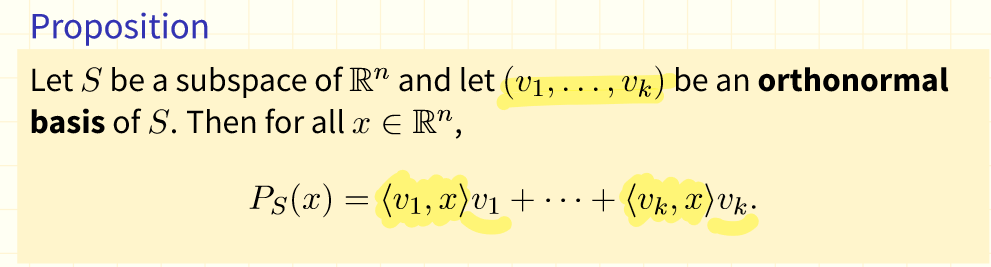
\includegraphics[scale=.45]{screenshots/computing orthogonal projection.png}\\

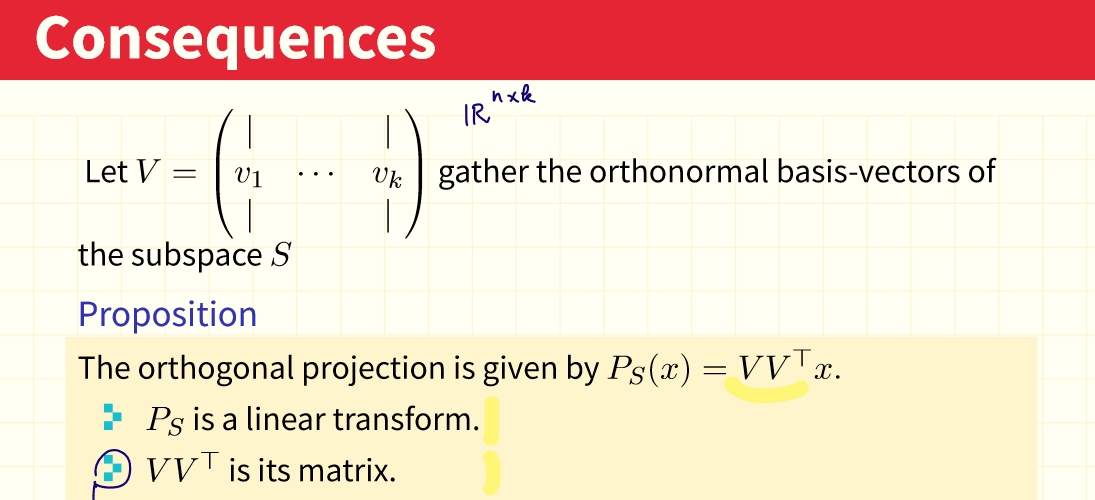
\includegraphics[scale=.45]{screenshots/consequences of orthogonal projection.png}

\section{Proofs:}

\begin{figure}[h]
    \centering
    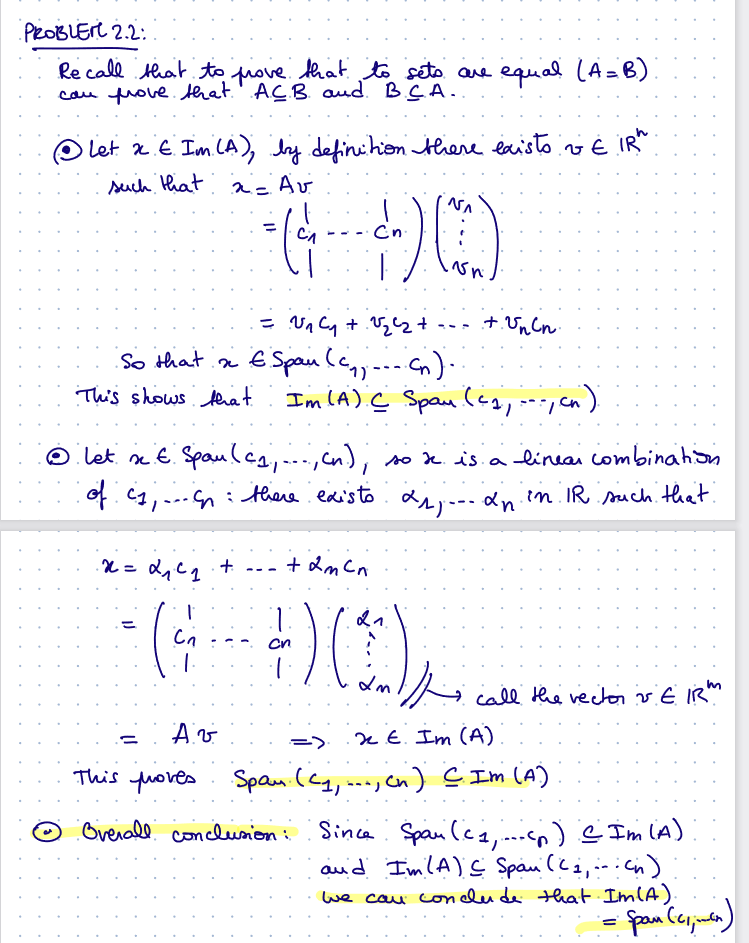
\includegraphics[scale=.7]{screenshots/Im(A) = span of columns proof.png}
    \caption{Im(A) = span of columns proof}
    \label{fig:my_label}
\end{figure}

\begin{figure}[h]
    \centering
    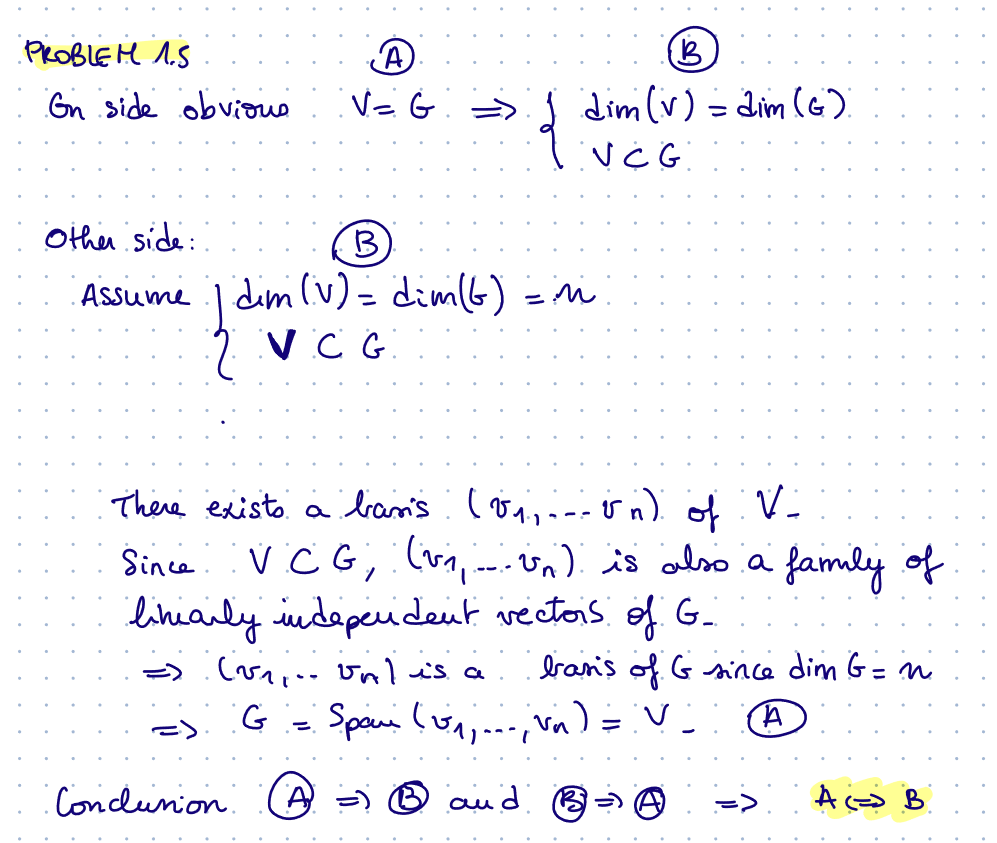
\includegraphics[scale=.45]{screenshots/proof subspaces are the same example 2.png}
    \caption{subspaces are the same example 2}
    \label{fig:my_label}
\end{figure}

\begin{figure}[h]
    \centering
    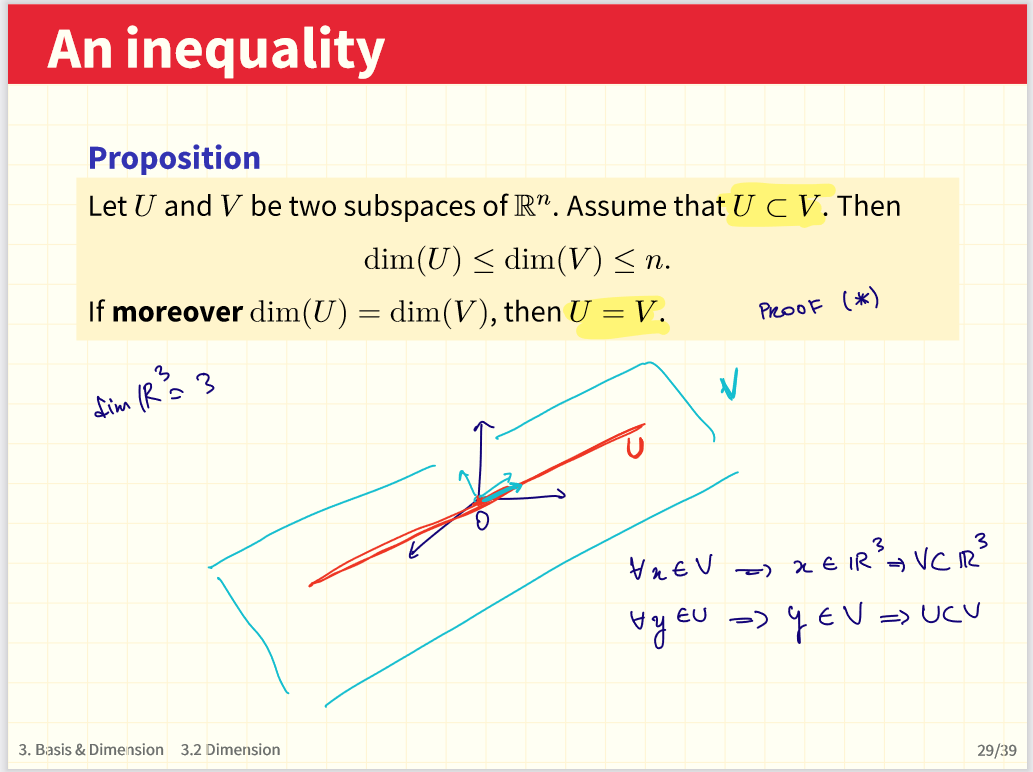
\includegraphics[scale=.45]{screenshots/subspaces are the same.png}
    \caption{subspaces are the same}
    \label{fig:my_label}
\end{figure}

\begin{figure}[h]
    \centering
    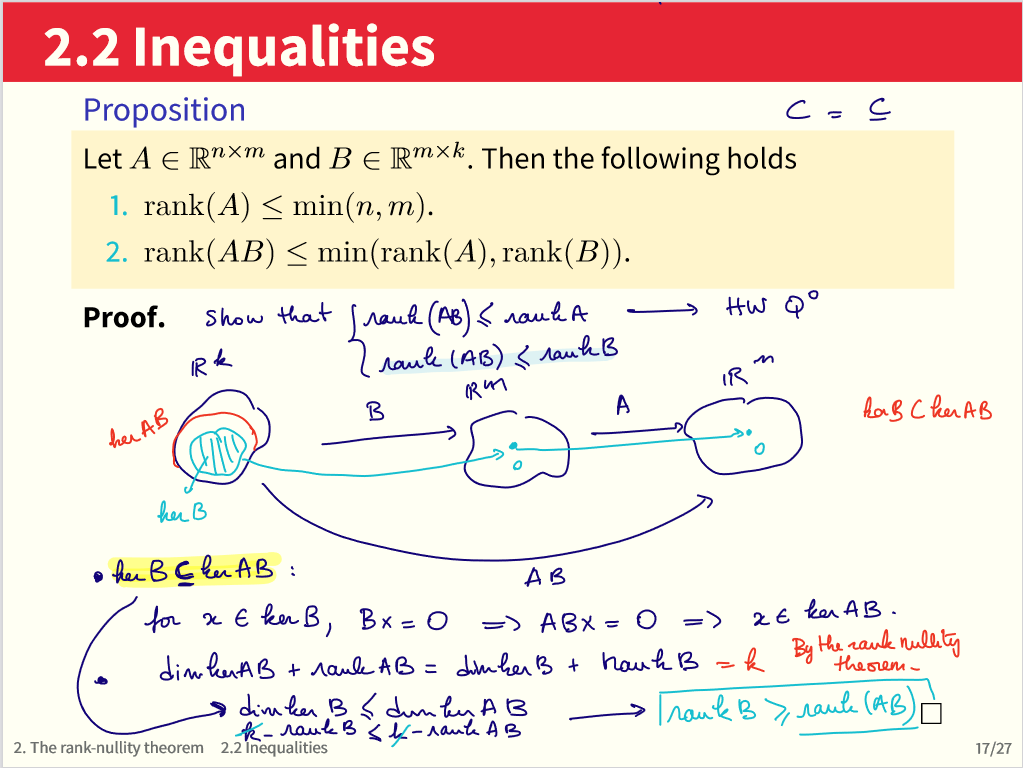
\includegraphics[scale=.45]{screenshots/rank nullity p1.png}
    \caption{rank nullity}
    \label{fig:my_label}
\end{figure}

\begin{figure}[h]
    \centering
    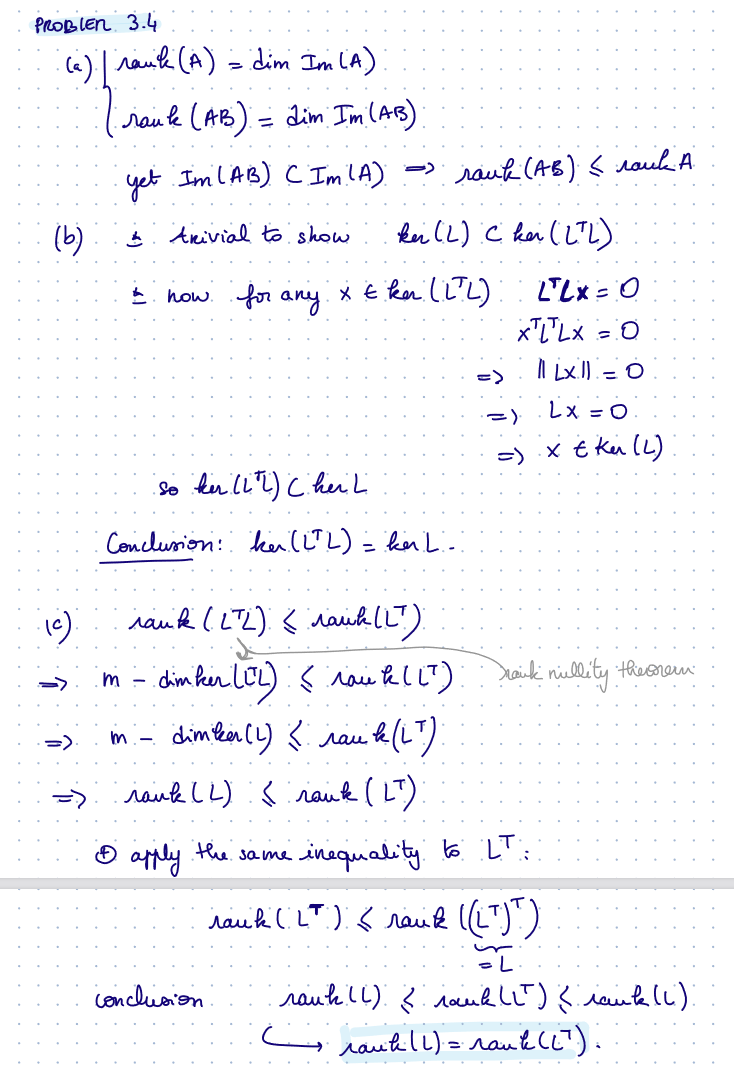
\includegraphics[scale=.7]{screenshots/rank L = rank LT proof.png}
    \caption{rank L = rank LT proof}
    \label{fig:my_label}
\end{figure}

\begin{figure}[h]
    \centering
    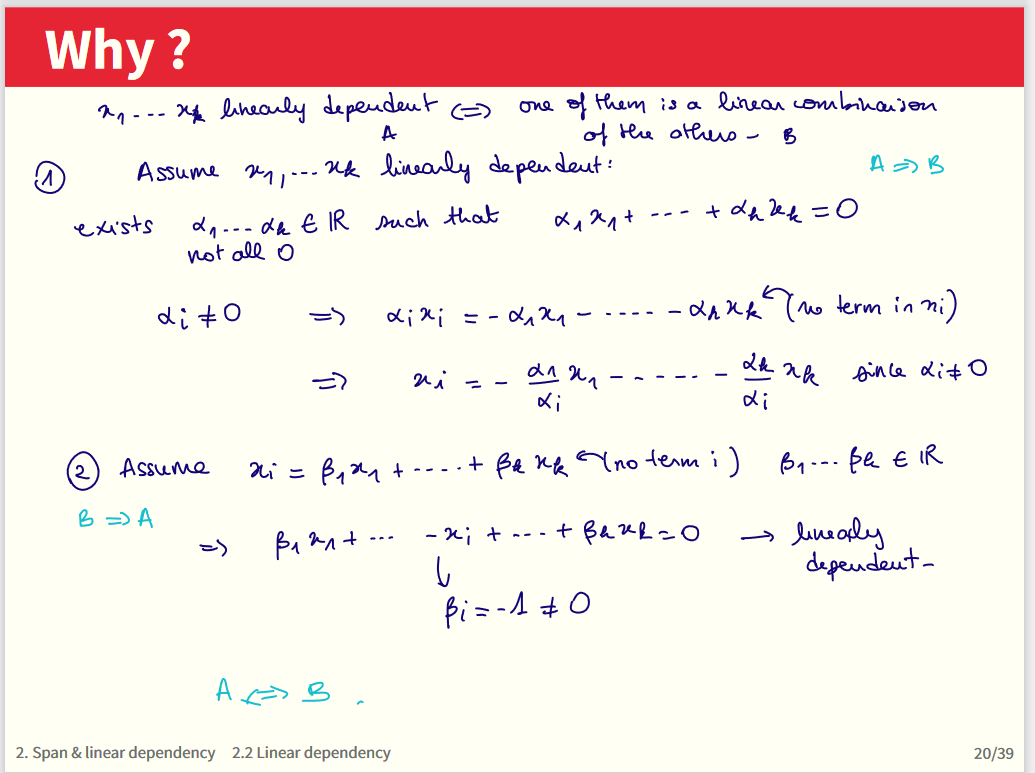
\includegraphics[scale=.45]{screenshots/how to prove linear dependence.png}
    \caption{how to prove linear dependence.png}
    \label{fig:my_label}
\end{figure}

\begin{figure}[h]
    \centering
    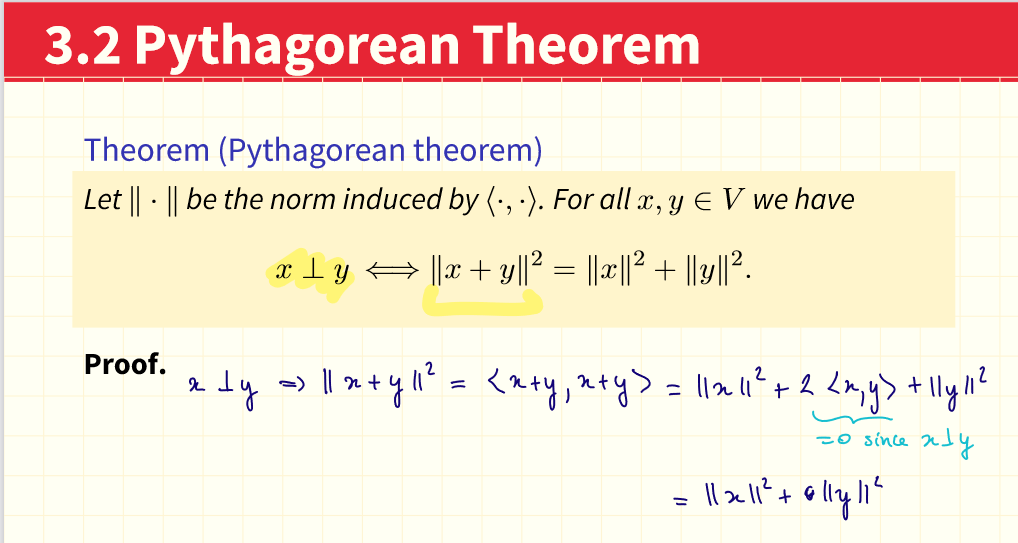
\includegraphics[scale=.45]{screenshots/pythagorean theorem.png}
    \caption{pythagorean theorem}
    \label{fig:my_label}
\end{figure}
\begin{figure}[h]
    \centering
    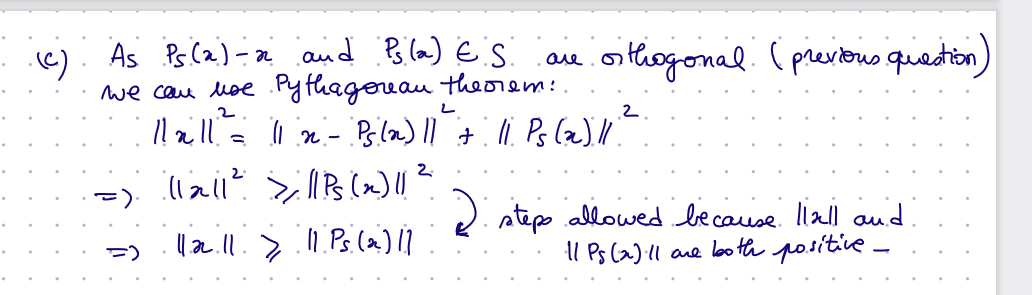
\includegraphics[scale=.45]{screenshots/norm of proj x leq norm of x.png}
    \caption{norm of proj x leq norm of x}
    \label{fig:my_label}
\end{figure}
\begin{figure}[h]
    \centering
    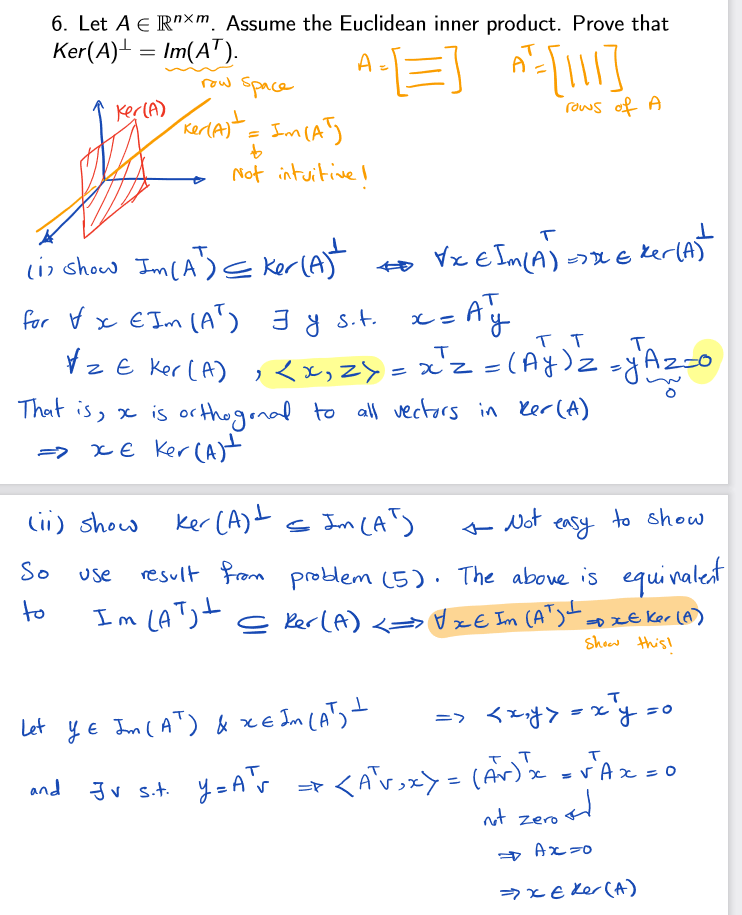
\includegraphics[scale=.7]{screenshots/complement to ker(a) = im(a^t).png}
    \caption{complement to ker(a) = im(a^t)}
    \label{fig:my_label}
\end{figure}
\begin{figure}[h]
    \centering
    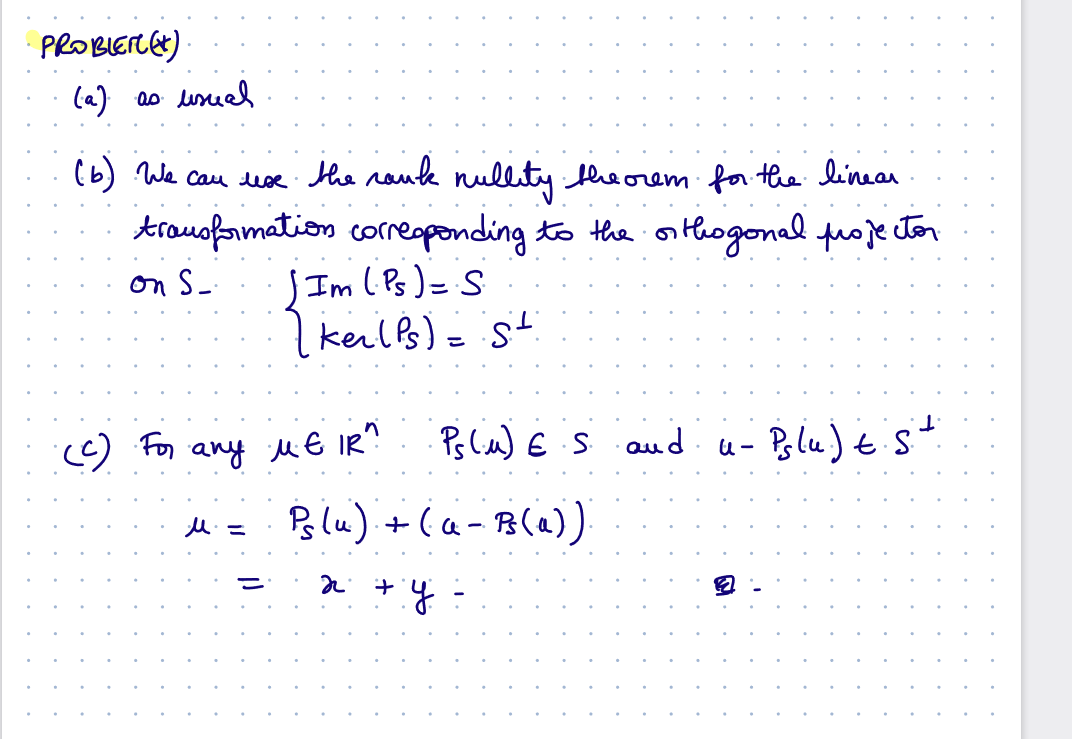
\includegraphics[scale=.45]{screenshots/dim s complement stuff (not that great tbh).png}
    \caption{dim s complement stuff (not that great tbh)}
    \label{fig:my_label}
\end{figure}

\begin{figure}[h]
    \centering
    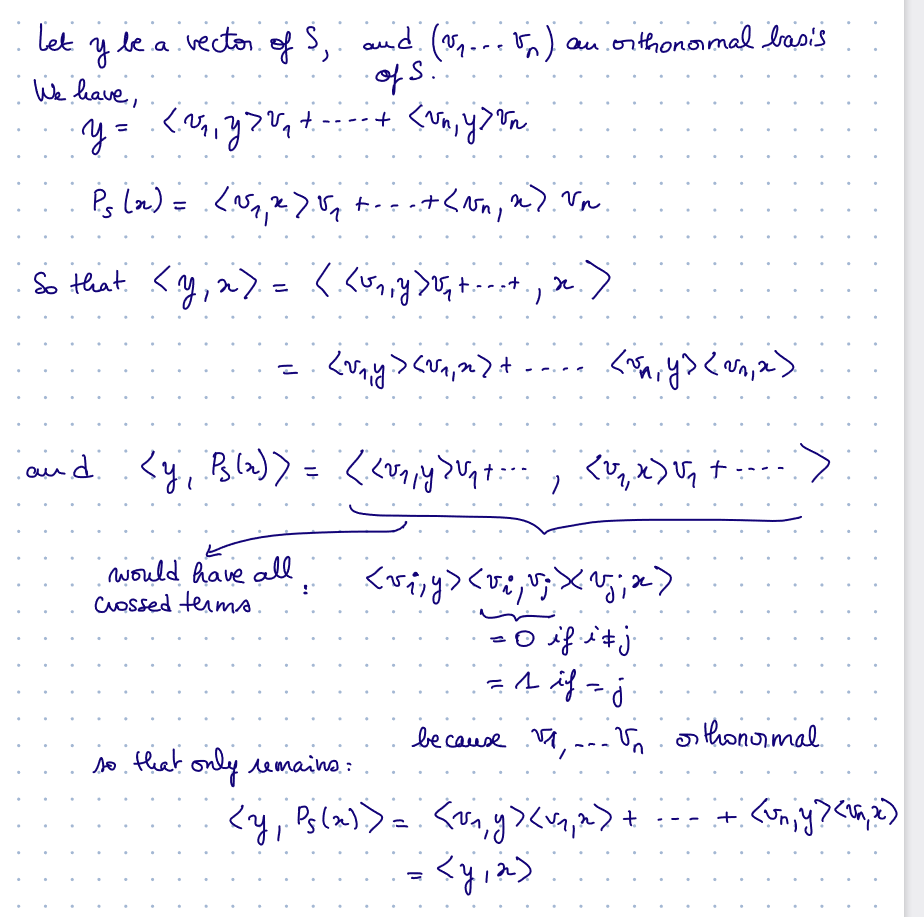
\includegraphics[scale=.45]{screenshots/dot of xy equals dot of projection x dot y.png}
    \caption{dot product of xy}
    \label{fig:my_label}
\end{figure}

\begin{figure}[h]
    \centering
    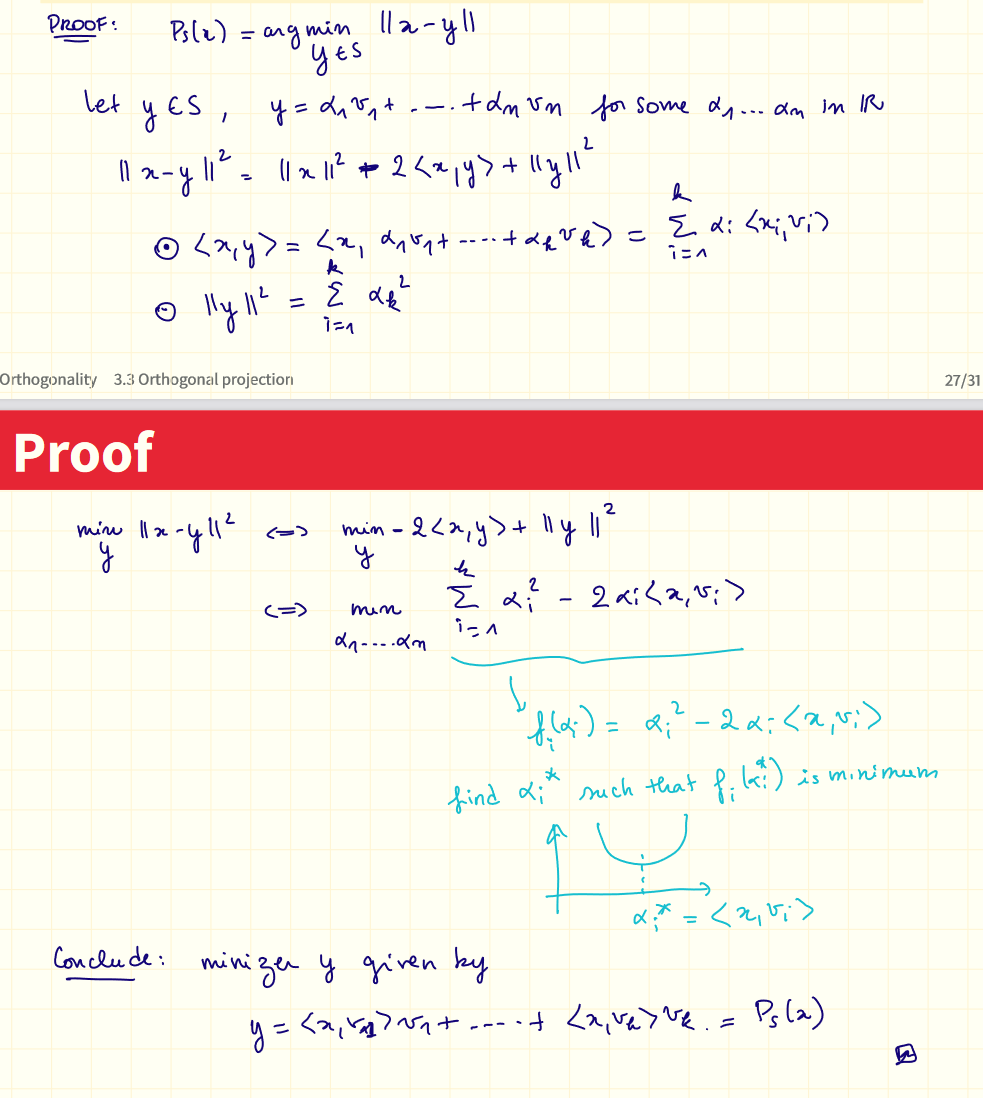
\includegraphics[scale=.65]{argmin projection proof.png}
    \caption{argmin projection proof}
    \label{fig:my_label}
\end{figure}













\end{document}
